\documentclass{article}
\usepackage[backend=biber,natbib=true,style=alphabetic,maxbibnames=50]{biblatex}
\addbibresource{/home/nqbh/reference/bib.bib}
\usepackage[utf8]{vietnam}
\usepackage{tocloft}
\renewcommand{\cftsecleader}{\cftdotfill{\cftdotsep}}
\usepackage[colorlinks=true,linkcolor=blue,urlcolor=red,citecolor=magenta]{hyperref}
\usepackage{amsmath,amssymb,amsthm,float,graphicx,mathtools,tikz}
\usetikzlibrary{angles,calc,intersections,matrix,patterns,quotes,shadings}
\allowdisplaybreaks
\newtheorem{assumption}{Assumption}
\newtheorem{baitoan}{}
\newtheorem{cauhoi}{Câu hỏi}
\newtheorem{conjecture}{Conjecture}
\newtheorem{corollary}{Corollary}
\newtheorem{dangtoan}{Dạng toán}
\newtheorem{definition}{Definition}
\newtheorem{dinhly}{Định lý}
\newtheorem{dinhnghia}{Định nghĩa}
\newtheorem{example}{Example}
\newtheorem{ghichu}{Ghi chú}
\newtheorem{hequa}{Hệ quả}
\newtheorem{hypothesis}{Hypothesis}
\newtheorem{lemma}{Lemma}
\newtheorem{luuy}{Lưu ý}
\newtheorem{nhanxet}{Nhận xét}
\newtheorem{notation}{Notation}
\newtheorem{note}{Note}
\newtheorem{principle}{Principle}
\newtheorem{problem}{Problem}
\newtheorem{proposition}{Proposition}
\newtheorem{question}{Question}
\newtheorem{remark}{Remark}
\newtheorem{theorem}{Theorem}
\newtheorem{vidu}{Ví dụ}
\usepackage[left=1cm,right=1cm,top=5mm,bottom=5mm,footskip=4mm]{geometry}
\def\labelitemii{$\circ$}
\DeclareRobustCommand{\divby}{%
	\mathrel{\vbox{\baselineskip.65ex\lineskiplimit0pt\hbox{.}\hbox{.}\hbox{.}}}%
}

\title{Problem: Cylinder, Cone, Sphere -- Bài Tập: Hình Trụ, Hình Nón, Hình Cầu}
\author{Nguyễn Quản Bá Hồng\footnote{e-mail: \texttt{nguyenquanbahong@gmail.com}, website: \url{https://nqbh.github.io}. Ben Tre City, Vietnam.}}
\date{\today}

\begin{document}
\maketitle
\begin{abstract}
	Latest version:
	\begin{itemize}
		\item \textit{Problem: Cylinder, Cone, Sphere -- Bài Tập: Hình Trụ, Hình Nón, Hình Cầu}.\\{\sc url}: \url{https://github.com/NQBH/elementary_STEM_beyond/blob/main/elementary_mathematics/grade_9/cylinder_cone_sphere/problem/NQBH_cylinder_cone_sphere_problem.pdf}.
		\item \textit{Problem \& Solution: Cylinder, Cone, Sphere -- Bài Tập \& Lời Giải: Hình Trụ, Hình Nón, Hình Cầu}.\\{\sc url}: \url{https://github.com/NQBH/elementary_STEM_beyond/blob/main/elementary_mathematics/grade_9/cylinder_cone_sphere/solution/NQBH_cylinder_cone_sphere_solution.pdf}.
	\end{itemize}
\end{abstract}
\tableofcontents

%------------------------------------------------------------------------------%

\section{Cylinder -- Hình Trụ}

\begin{center}
	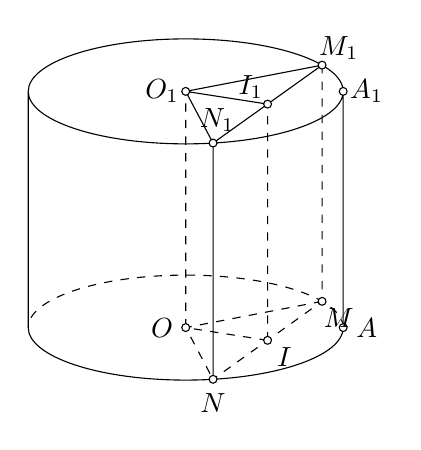
\begin{tikzpicture}
		\def\r{2}
		\def\h{3}
		\def\gM{30}
		\def\gN{-80}
		\path
		(0:0) coordinate (O)
		(0:\r) coordinate (A)
		(180:\r) coordinate (B)
		(A) arc (0:\gM:{\r} and {\r/3}) coordinate (M)
		(A) arc (0:\gN:{\r} and {\r/3}) coordinate (N)
		($(M)!.5!(N)$) coordinate (I)
		\foreach \x in {O,A,B,M,N,I}{(\x)++(90:\h) coordinate (\x_1)};
		\draw[dashed]
		(I)--(O)--(O_1) (M)--(O)--(N) (M_1)--(M)--(N) (I)--(I_1) (A) arc (0:180:{\r} and {\r/3});
		\draw (A) arc (0:-180:{\r} and {\r/3}) (O_1) ellipse ({\r} and {\r/3}) (A)--(A_1) (B)--(B_1) (N)--(N_1) (O_1)--(I_1) (O_1)--(M_1)--(N_1)--cycle;
		\foreach \x/\g in {A/0,A_1/0,O/180,O_1/180,I/-45,M/-45,N/-90,M_1/45,N_1/80,I_1/135} \draw[fill=white] (\x) circle (.05) + (\g:.3) node{$\x$};
	\end{tikzpicture}
\end{center}
\fbox{1} Quay hình chữ nhật $ABCD$ 1 vòng quanh cạnh $CD$ cố định (trục quay) được 1 hình trụ với 2 đáy: 2 hình tròn $(C;R),(D;R)$ với $R = AD = BC$, mặt xung quanh, đường sinh $AB$, chiều cao $AB = h$. \fbox{2} {\sf Thiết diện}: \textit{Mặt cắt song song với đáy}: Thiết diện là 1 hình tròn bằng đáy. \textit{Mặt cắt song song với trục}: Thiết diện là 1 hình chữ nhật. \fbox{3} Hình trụ có diện tích xung quanh \fbox{$S_{\rm xq} = 2\pi Rh$}, diện tích toàn phần \fbox{$S_{\rm tp} = 2\pi Rh + 2\pi R^2$}, thể tích \fbox{$V = S_{\scriptsize\mbox{\rm đ}}h = \pi R^2h$}.\\
\\
\cite[Chap. X, \S1, pp. 92--97]{SGK_Toan_9_Canh_Dieu_tap_1}: HD1. HD2. LT1. HD3. LT2. HD4. 1. 2. 3. 4. 5. 6.

\begin{baitoan}[{\sf Program}: Cylinder]
	Cho 2 trong 6 yếu tố: $R,h,S_{\rm xq},S_{\scriptsize\mbox{\rm đ}},S_{\rm tp},V$, tìm 4 yếu tố còn lại của hình trụ theo 2 yếu tố cho trước. Viết chương trình {\sf Pascal, Python, C{\tt/}C++} để minh họa.
\end{baitoan}

\begin{baitoan}[\cite{Binh_boi_duong_Toan_9_tap_2}, H1, p. 114]
	Nếu tăng bán kính đáy của hình trụ lên gấp đôi, gấp $a$ lần thì diện tích xung quanh, diện tích toàn phần, thể tích của hình trụ tăng mấy lần?
\end{baitoan}

\begin{baitoan}[\cite{Binh_boi_duong_Toan_9_tap_2}, H2, p. 114]
	Nếu giảm chiều cao của hình trụ đi $2$ lần, a lần thì thể tích hình trụ giảm đi mấy lần?
\end{baitoan}

\begin{baitoan}[\cite{Binh_boi_duong_Toan_9_tap_2}, H3, p. 114]
	Có 2 cốc hình trụ, cốc to có chiều cao gấp rưỡi chiều cao cốc nhỏ \& đường kính đáy gấp đôi đường kính đáy cốc nhỏ. Phải đong đầy bao nhiêu cốc nước nhỏ để đổ đầy được cốc to?
\end{baitoan}

\begin{baitoan}[\cite{Binh_boi_duong_Toan_9_tap_2}, VD1, p. 115]
	Cắt hình trụ bằng 1 mặt phẳng chứa trục. Biết thiết diện là 1 hình vuông có diện tích bằng $S = 36\ {\rm cm}^2$. Tính diện tích xung quanh, diện tích toàn phần, \& thể tích hình trụ.
\end{baitoan}

\begin{baitoan}[\cite{Binh_boi_duong_Toan_9_tap_2}, VD2, p. 115]
	1 hình trụ có chu vi đáy $P = 24\pi$ {\rm cm} \& diện tích toàn phần là $S = 768\pi\ {\rm cm}^2$. Tính thể tích hình trụ.
\end{baitoan}

\begin{baitoan}[\cite{Binh_boi_duong_Toan_9_tap_2}, VD3, p. 115]
	1 hộp sữa hình trụ có chiều cao hơn đường kính đáy là $a = 3$ {\rm cm}. Biết diện tích vỏ hộp (kể cả nắp) là $S = 292.5\pi\ {\rm cm}^2$. Tính thể tích hộp sữa đó.
\end{baitoan}

\begin{baitoan}[\cite{Binh_boi_duong_Toan_9_tap_2}, VD4, p. 116]
	1 hình trụ có bán kính đáy R \& chiều cao $2R$. Vẽ 1 đường sinh AB cố định. Lấy điểm M trên đường tròn đáy có chứa A \& đặt $\widehat{ABM} = \alpha$. Tìm giá trị của $\alpha$ để độ dài BM lớn nhất. Tính {\rm GTLN} đó.
\end{baitoan}
{\sf Hint.} Trong hình trụ, đường sinh vuông góc với đáy nên vuông góc với mọi đường thẳng nằm trong đáy.

\begin{baitoan}[\cite{Binh_boi_duong_Toan_9_tap_2}, VD5, p. 116]
	1 con kiến bò trên mặt ngoài 1 cái cốc hình trụ từ A ở mép dưới để đến M ở mép trên. AB là đường sinh đi qua A. $AB = a = 15$ {\rm cm}, $\widehat{BOM} = \alpha = 105^\circ$, \& bán kính đáy hộp là $r = 6$ {\rm cm}. Tính độ dài ngắn nhất mà kiến phải bò.
\end{baitoan}

\begin{baitoan}[\cite{Binh_boi_duong_Toan_9_tap_2}, 8.1., p. 117]
	1 hình trụ có chiều cao $h = 5$ {\rm cm}. Biết diện tích toàn phần gấp đôi diện tích xung quanh. Tính thể tích hình trụ.
\end{baitoan}

\begin{baitoan}[\cite{Binh_boi_duong_Toan_9_tap_2}, 8.2., p. 117]
	1 thùng phuy hình trụ có số đo $\rm m^2$ diện tích xung quanh đúng bằng số đo $\rm m^3$ thể tích. Tính bán kính đáy của thùng.
\end{baitoan}

\begin{baitoan}[\cite{Binh_boi_duong_Toan_9_tap_2}, 8.3., p. 117]
	Tỷ số giữa diện tích xung quanh \& diện tích toàn phần của 1 hình trụ là $a = \frac{3}{5}$. Biết bán kính đáy $r = 6$ {\rm cm}, tính chiều cao hình trụ.
\end{baitoan}

\begin{baitoan}[\cite{Binh_boi_duong_Toan_9_tap_2}, 8.4., p. 117]
	1 hình trụ có thể tích $V = 300\ {\rm cm}^3$ \& diện tích xung quanh $S = 120\ {\rm cm}^2$. Tính diện tích toàn phần hình trụ.
\end{baitoan}

\begin{baitoan}[\cite{Binh_boi_duong_Toan_9_tap_2}, 8.5., p. 117]
	1 hình trụ có diện tích xung quanh $s = 24\pi\ {\rm cm}^2$ \& diện tích toàn phần $S = 42\pi\ {\rm cm}^2$. Tính thể tích hình trụ.
\end{baitoan}

\begin{baitoan}[\cite{Binh_boi_duong_Toan_9_tap_2}, 8.6., p. 117]
	1 hình trụ có đường kính đáy bằng $a = \frac{2}{3}$ chiều cao. Cắt hình trụ này bằng 1 mặt phẳng chứa trục ta được 1 hình chữ nhật có diện tích $S = 54\ {\rm cm}^2$. Tính diện tích xung quanh của hình trụ.
\end{baitoan}

\begin{baitoan}[\cite{Binh_boi_duong_Toan_9_tap_2}, 8.7., p. 117]
	1 chai thủy tinh dung tích $V = 0.75$ {\rm l} có phần dưới là hình trụ. Trong chai có nước đến độ cao $h = 10.3$ {\rm cm} \& được đánh dấu bằng 1 vạch đỏ. Nút kín rồi bậc ngược chai thì mực nước vẫn đúng vạch đỏ. Tính bán kính đáy chai (phần bên trong chai).
\end{baitoan}

\begin{baitoan}[\cite{Binh_boi_duong_Toan_9_tap_2}, 8.8., p. 117]
	1 hình trụ có chiều cao $h = 18$ {\rm cm} \& diện tích toàn phần $S = 176\pi\ {\rm cm}^2$. (a) Chứng minh diện tích xung quanh hình trụ bằng $9$ lần diện tích đáy. (b) Tính tỷ số $\dfrac{S_{\rm xq}}{S_{\tiny\mbox{\rm đ}}}$ trong trường hợp tổng quát.
\end{baitoan}

\begin{baitoan}[\cite{Binh_boi_duong_Toan_9_tap_2}, 8.9., p. 117]
	1 lọ hình trụ được ``đặc khít'' trong 1 hộp giấy hình hộp chữ nhật. Biết thể tích của lọ hình trụ là $V = 270\ {\rm cm}^3$, tính thể tích hộp giấy.
\end{baitoan}

\begin{baitoan}[\cite{Binh_boi_duong_Toan_9_tap_2}, 8.10., p. 117]
	1 hình lăng trụ đứng có chiều cao $h = 5$ {\rm cm}. Đáy của lăng trụ là 1 tam giác vuông có 2 cạnh góc vuông dài $b = 6$ {\rm cm}, $c = 8$ {\rm cm}. Tính thể tích hình trụ nội tiếp hình lăng trụ này.
\end{baitoan}

\begin{baitoan}[\cite{Binh_boi_duong_Toan_9_tap_2}, p. 118]
	1 chiếc cốc thủy tinh hình trụ đựng đầy sữa. Tìm cách để rót ra đúng 1 nửa cốc sữa.
\end{baitoan}

\begin{baitoan}[\cite{Binh_boi_duong_Toan_9_tap_2}, p. 118]
	Vì sao phích nước, bể chứa xăng đều là hình trụ?
\end{baitoan}

\begin{baitoan}[\cite{Binh_boi_duong_Toan_9_tap_2}, p. 118]
	Vì sao bể (có nắp) chứa chất lỏng hình trụ có đường kính bằng chiều cao thì tốn ít vật liệu nhất?
\end{baitoan}

\begin{baitoan}[\cite{Tuyen_Toan_9_old}, VD29, p. 158]
	1 hình trụ có thiết diện qua trục là 1 hình vuông. Biết thể tích hình trụ là $128\pi\ {\rm cm}^3$. (a) Tính bán kính đáy. (b) Tính tỷ số giữa diện tích xung quanh \& diện tích toàn phần.
\end{baitoan}

\begin{baitoan}[\cite{Tuyen_Toan_9_old}, 156., p. 159]
	1 thùng hình trụ có diện tích xung quanh bằng $\frac{1}{2}$ diện tích toàn phần. Biết bán kính đáy là {\rm40 cm}, tính dung tích của thùng.
\end{baitoan}

\begin{baitoan}[\cite{Tuyen_Toan_9_old}, 157., p. 159]
	1 hình trụ có bán kính đáy là {\rm5 cm}, có thể tích là $200\pi\ {\rm cm}^3$. (a) Tính diện tích của thiết diện qua trục. (b) Thiết diện $ABB'A'$ song song với trục $OO'$, AB là dây cung của đường tròn tâm O. Tính khoảng cách từ O đến AB để cho thiết diện đó là 1 hình vuông.
\end{baitoan}

\begin{baitoan}[\cite{Tuyen_Toan_9_old}, 158., p. 160]
	Từ 1 tấm tôn hình chữ nhật có kích thước $ab$, $a > b$, cuốn lại thành mặt xung quanh của 1 hình trụ. Phải cuốn theo chiều nào của tấm tôn để được 1 hình trụ không đáy có thể tích lớn nhất?
\end{baitoan}

\begin{baitoan}[\cite{Tuyen_Toan_9_old}, 159., p. 160]
	Muốn sản xuất 1 loại thùng phuy hình trụ chứa xăng dầu có thể tích V cho trước. Tìm mối quan hệ giữa chiều cao h \& bán kính R để tốn ít vật liệu nhất.
\end{baitoan}

\begin{baitoan}[\cite{Tuyen_Toan_9_old}, 160., p. 160]
	Muốn làm 1 thùng tôn hình trụ không có nắp để đựng nước, chứa được $\approx8\pi$ {\rm l} nước. Phải làm chiếc thùng đó có chiều cao \& bán kính đáy là bao nhiêu để tồn ít vật liệu nhất?
\end{baitoan}

\begin{baitoan}[\cite{Binh_Toan_9_tap_2}, VD46, p. 114]
	1 chai nước có phía dưới là hình trụ chứa 1 lượng nước có chiều cao {\rm10 cm}. Lật ngược chai lại thì phần chai không chứa nước là 1 hình trụ có chiều cao {\rm8 cm}. Tính thể tích của chai, biết đường kính của đáy chai bằng {\rm10 cm}.
\end{baitoan}

\begin{baitoan}[\cite{Binh_Toan_9_tap_2}, 341., p. 114]
	Có 3 vật hình trụ bằng chì, bằng sắt, bằng nhôm cùng có khối lượng bằng {\rm2 kg} \& cùng có đường kính đáy bằng {\rm10 cm}. Tính chiều cao của mỗi vật, biết khối lượng riêng của chì là {\rm11.3 kg{\tt/}$\rm dm^3$}, khối lượng riêng của sắt là {\rm7.8 kg{\tt/}$\rm dm^3$}, khối lượng riêng của nhôm là {\rm2.7 kg{\tt/}$\rm dm^3$}.
\end{baitoan}

\begin{baitoan}[\cite{Binh_Toan_9_tap_2}, 342., p. 114]
	1 băng giấy dải được cuộn chặt lại $60$ vòng làm thành 1 cuộn giấy hình trụ rỗng. Biết đường kính của đường tròn trong cùng bằng {\rm2 cm}, đường kính của đường tròn ngoài cùng bằng {\rm6 cm}. Tính chiều cao của băng giấy.
\end{baitoan}

\begin{baitoan}[\cite{Binh_Toan_9_tap_2}, 343., p. 114]
	Cần cưa 1 thân cây hình trụ có đường kính đáy bằng $d$ để được 1 khúc gỗ hình chữ nhật có thể tích lớn nhất. Tính các kích thước đáy của khúc gỗ hình hộp chữ nhật.
\end{baitoan}

\begin{baitoan}[\cite{Binh_Toan_9_tap_2}, 344., p. 114, Kiến \& mật]
	1 con kiến ở vị trí A trên mặt ngoài của 1 lọ thủy tinh hình trụ không có nắp, nhìn thấy 1 giọt mật ở thẳng trước mặt tại vị trí B ở mặt trong của lọ. Biết A cách miệng lọ {\rm5 cm}, B cách miệng lọ {\rm2 cm}, \& độ dài của đường tròn miệng lọ bằng {\rm48 cm}. Tính độ dài ngắn nhất để chú kiến bò được tới chỗ giọt mật.
\end{baitoan}

\begin{baitoan}[\cite{Binh_Toan_9_tap_2}, 345., p. 114]
	Chứng minh trong các hình trụ có cùng thể tích, hình trụ có đường cao bằng đường kính của đáy là hình có diện tích toàn phần nhỏ nhất.
\end{baitoan}

%------------------------------------------------------------------------------%

\section{Cone -- Hình Nón}
\begin{center}
	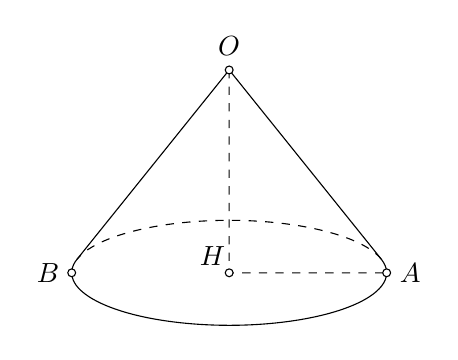
\begin{tikzpicture}
		\def\r{2}
		\def\gM{15}
		\path
		(0:0) coordinate (H)
		(0:\r) coordinate (A)
		(180:\r) coordinate (B)
		(A) arc (0:\gM:{\r} and {\r/3}) coordinate (M)--([turn]0:1mm) coordinate (Mt)
		(B) arc (180:180-\gM:{\r} and {\r/3}) coordinate (M')--([turn]0:1mm) coordinate (M't)
		(intersection of M--Mt and M'--M't) coordinate (O);
		\draw[dashed] (O)--(H)--(A) (M) arc (\gM:180-\gM:{\r} and {\r/3});
		\draw (M') arc (180-\gM:360+\gM:{\r} and {\r/3}) (M)--(O)--(M');
		\foreach \x/\g in {A/0,B/180,O/90,H/135} \draw[fill=white] (\x) circle (.05) + (\g:.3) node{$\x$};
	\end{tikzpicture}
\end{center}
\fbox{1} Quy $\Delta AOB$ vuông tại $O$ 1 vòng quành cạnh góc vuông $OA$ cố định được 1 hình nón có đáy: hình tròn $(O;R)$, đỉnh $A$, mặt xung quanh, đường sinh $AB = l$, chiều cao $AO = h$. \fbox{2} Hình nón có diện tích xung quanh \fbox{$S_{\rm xq} = \pi Rl$}, diện tích toàn phần \fbox{$S_{\rm tp} = \pi Rl + \pi R^2$}, thể tích \fbox{$V = \frac{1}{3}S_{\scriptsize\mbox{\rm đ}}h = \frac{1}{3}\pi R^2h$}. \fbox{3} Hình nón cụt với 2 đáy $(O';r),(O;R)$ có diện tích xung quanh \fbox{$S_{\rm xq} = \pi(R + r)l$}, diện tích toàn phần \fbox{$S_{\rm tp} = \pi(R + r)l + \pi(R^2 + r^2)$}, thể tích \fbox{$V = \frac{1}{3}\pi h(R^2 + Rr + r^2)$}.\\
\\
\cite[Chap. X, \S2, pp. 98--103]{SGK_Toan_9_Canh_Dieu_tap_1}: HD1. HD2. LT1. HD3. LT2. HD4. 1. 2. 3. 4.

\begin{baitoan}[{\sf Program}: Cone]
	Cho 2 trong 7 yếu tố: $R,l,h,S_{\rm xq},S_{\scriptsize\mbox{\rm đ}},S_{\rm tp},V$, tìm 5 yếu tố còn lại của hình nón theo 2 yếu tố cho trước. Viết chương trình {\sf Pascal, Python, C{\tt/}C++} để minh họa.
\end{baitoan}

\begin{baitoan}[{\sf Program}: Truncated cone]
	Cho 3 trong 8 yếu tố: $R,r,l,h,S_{\rm xq},S_{\scriptsize\mbox{\rm đ}},S_{\rm tp},V$, tìm 5 yếu tố còn lại của hình nón cụt theo 2 yếu tố cho trước. Viết chương trình {\sf Pascal, Python, C{\tt/}C++} để minh họa.
\end{baitoan}

\begin{baitoan}[\cite{Binh_boi_duong_Toan_9_tap_2}, H1, p. 120]
	1 hình trụ \& 1 hình nón có chung đáy, chiều cao bằng nhau, tính tỷ số thể tích của chúng.
\end{baitoan}

\begin{baitoan}[\cite{Binh_boi_duong_Toan_9_tap_2}, H2, p. 120]
	Cho $\Delta ABO$ vuông tại O. Biết $OA = a = 3$ {\rm cm}, $OB = b = 2$ {\rm cm}. So sánh thể tích của 2 hình nón tạo thành khi quay tam giác 1 vòng lần lượt quanh cạnh OA \& cạnh OB.
\end{baitoan}

\begin{baitoan}[\cite{Binh_boi_duong_Toan_9_tap_2}, H3, p. 120]
	Tính đường sinh của 1 hình nón có bán kính đáy $r = 21$ {\rm cm} \& chiều cao $h = 17$ {\rm cm}.
\end{baitoan}

\begin{baitoan}[\cite{Binh_boi_duong_Toan_9_tap_2}, VD1, p. 120]
	1 hình nón có bán kính đáy bằng $r = 20$ {\rm cm} \& diện tích xung quanh bằng $S = 580\pi\ {\rm cm}^2$. Tính thể tích hình nón.
\end{baitoan}

\begin{baitoan}[\cite{Binh_boi_duong_Toan_9_tap_2}, VD2, p. 120]
	1 hình nón có bán kính đáy $r = 5$ {\rm cm}, đường sinh $l = 12$ {\rm cm}. Khai triển hình nón này theo 1 đường sinh rồi trải phẳng ra ta được 1 hình quạt tròn. Tính số đo cung của hình quạt tròn.
\end{baitoan}

\begin{baitoan}[\cite{Binh_boi_duong_Toan_9_tap_2}, VD3, p. 121]
	1 chiếc xô nhỏ đựng nước hình nón cụt làm bằng tôn. 2 bán kính đáy lần lượt là $R = 11,r = 6$, chiều cao của xô $h = 12$. (a) Tính dung tích chiếc xô. (b) Tính diện tích tôn để làm xô (diện tích các mối ghép không đáng kể).
\end{baitoan}

\begin{baitoan}[\cite{Binh_boi_duong_Toan_9_tap_2}, VD4, p. 122]
	Cho 1 hình nón đỉnh A, đường kính đáy $BC = R = 4$, đường sinh $AB = l = 6$. Khai triển mặt xung quanh của hình nón theo đường sinh AB ta được 1 hình quạt tròn. (a) Tính số đo cung của hình quạt đó. (b) Tính quãng đường ngắn nhất mà con kiến bò trên mặt xung quanh của hình nón từ B đến C.
\end{baitoan}

\begin{baitoan}[\cite{Binh_boi_duong_Toan_9_tap_2}, 9.1., p. 122]
	1 hình quạt tròn bán kính $R = 20$ \& góc ở tâm là $\alpha = 108^\circ$. Cuốn hình quạt này thành mặt xung quanh của 1 hình nón. Tính chiều cao của hình nón này.
\end{baitoan}

\begin{baitoan}[\cite{Binh_boi_duong_Toan_9_tap_2}, 9.2., p. 122]
	1 hình nón có bán kính đáy $r = 5$, chiều cao $h = \frac{3}{4}$ bán kính đáy. Chứng minh số đo diện tích xung quanh $\rm cm^2$ bằng số đo thể tích $\rm cm^3$.
\end{baitoan}

\begin{baitoan}[\cite{Binh_boi_duong_Toan_9_tap_2}, 9.3., p. 122]
	1 hình nón có đáy là hình tròn ngoại tiếp hình vuông cạnh $a = 3\sqrt{2}$. Biết chiều cao hình nón $h = 4$, tính diện tích xung quanh \& thể tích hình nón.
\end{baitoan}

\begin{baitoan}[\cite{Binh_boi_duong_Toan_9_tap_2}, 9.4., p. 122]
	1 hình nón có bán kính đáy R. Thiết diện chứa trục hình nón là 1 tam giác đều. (a) Chứng minh diện tích xung quanh của hình nón bằng $2$ lần diện tích đáy. (b) Tính thể tích hình nón.
\end{baitoan}

\begin{baitoan}[\cite{Binh_boi_duong_Toan_9_tap_2}, 9.5., p. 123]
	1 hình nón có thể tích bằng $\rm120\ cm^3$. Cắt hình nón này bằng 1 mặt phẳng song song với đáy \& đi qua trung điểm đường cao. Tính thể tích của hình nón cụt.
\end{baitoan}

\begin{baitoan}[\cite{Binh_boi_duong_Toan_9_tap_2}, 9.6., p. 123]
	1 hình nón cụt có 2 bán kính đáy là $r = 14,R = 26$. Biết diện tích xung quanh của nó là $\rm1480\pi\ cm^2$. Tính chiều cao, thể tích hình nón cụt.
\end{baitoan}

\begin{baitoan}[\cite{Binh_boi_duong_Toan_9_tap_2}, 9.7., p. 123]
	1 hình nón có bán kính đáy là $R = 18$ \& đường sinh $l = 40$. 1 mặt phẳng $(P)$ song song với đáy cắt mặt xung quanh của hình nón theo đường tròn $(O')$ chia mặt xung quanh của hình nón thành 2 phần có diện tích bằng nhau. Tính bán kính đường tròn $(O')$.
\end{baitoan}

\begin{baitoan}[\cite{Binh_boi_duong_Toan_9_tap_2}, 9.8., p. 123]
	Cho $\Delta ABC$ vuông tại A, $AB = c = 3,AC = b = 4$. Quay tam giác vuông này 1 vòng xung quanh cạnh BC cố định. Tính diện tích toàn phần, thể tích của hình tạo thành.
\end{baitoan}

\begin{baitoan}[\cite{Binh_boi_duong_Toan_9_tap_2}, 9.9., p. 123]
	Cho $\Delta ABC$, $\widehat{B}$ tù, $BC = a$, đường cao $AH = h$. Quay hình tam giác này 1 vòng quanh cạnh BC cố định. Tính thể tích của hình tạo thành.
\end{baitoan}

\begin{baitoan}[\cite{Binh_boi_duong_Toan_9_tap_2}, 9.10., p. 123]
	Cho hình thang ABCD có $\widehat{A} = \widehat{D} = 90^\circ$, $AB = a = 4,AD = b = 6,\widehat{C} = \alpha = 30^\circ$. Quay hình thang vuông này 1 vòng quanh cạnh CD cố định ta được 1 hình $(\mathcal{H})$. Tính thể tích hình $(\mathcal{H})$.
\end{baitoan}

\begin{baitoan}[\cite{Binh_boi_duong_Toan_9_tap_2}, p. 123, công thức tính thể tích hình nón]
	Chứng minh công thức tính thể tích hình nón bằng cách xem nó là giới hạn của thể tích hình chóp $n$-giác đều nội tiếp trong hình nón khi số cạnh $n\to\infty$.
\end{baitoan}

\begin{baitoan}[\cite{Tuyen_Toan_9_old}, VD30, p. 161]
	Mặt xung quanh của 1 hình nón khai triển thành 1 hình quạt $100^\circ48'$, bán kính {\rm25 cm}. Tính diện tích toàn phần \& thể tích hình nón đó.
\end{baitoan}

\begin{baitoan}[\cite{Tuyen_Toan_9_old}, 161., p. 162]
	Cho $\Delta ABC$ vuông tại C. Biết $BC = a,AC = b$. Quay tam giác vuông này 1 vòng lần lượt quanh cạnh $AC,BC$, được 1 hình nón đỉnh A \& 1 hình nón đỉnh B. So sánh tỷ số thể tích của 2 hình nón với tỷ số diện tích xung quanh của 2 hình nón ấy.
\end{baitoan}

\begin{baitoan}[\cite{Tuyen_Toan_9_old}, 162., p. 162]
	Từ 1 khúc gỗ hình trụ, tiện thành 1 hình nón có thể tích lớn nhất. Biết thể tích phần gỗ bị tiện bỏ đi là $200\pi\ {\rm cm}^3$. (a) Tính thể tích hình nón. (b) Giả sử chiều cao của hình nón là {\rm12 cm}. Tính diện tích xung quanh của hình nón.
\end{baitoan}

\begin{baitoan}[\cite{Tuyen_Toan_9_old}, 163., p. 162]
	1 hình nón có đường cao bằng h \& có thiết diện qua trục là 1 tam giác đều. (a) Chứng minh diện tích đáy bằng $\frac{1}{2}$ diện tích xung quanh. (b) Cắt hình nón bằng 1 nửa mặt phẳng song song với đáy tạo ra 1 hình nón cụt. Tính chiều cao của hình nón cụt biết diện tích xung quanh của nó bằng diện tích đáy lớn.
\end{baitoan}

\begin{baitoan}[\cite{Tuyen_Toan_9_old}, 164., p. 163]
	1 hình nón cụt có các bán kính đáy là $R = 20$ {\rm cm}, $r = 12$ {\rm cm}, \& đường cao $h = 15$ {\rm cm}. (a) Tính diện tích xung quanh của hình nón cụt. (b) Tính thể tích của hình nón sinh ra hình nón cụt đó.
\end{baitoan}

\begin{baitoan}[\cite{Tuyen_Toan_9_old}, 165., p. 163]
	1 hình nón cụt, bán kính đáy lớn bằng {\rm8 cm}, đường cao bằng {\rm12 cm}, \& đường sinh bằng {\rm13 cm}. (a) Tính bán kính đáy nhỏ. (b) Tính diện tích xung quanh \& thể tích của hình nón cụt đó.
\end{baitoan}

\begin{baitoan}[\cite{Binh_Toan_9_tap_2}, VD47, p. 115]
	Cho $\Delta OBC$ vuông tại O. Nếu quay tam giác đó quanh cạnh $OB$ cố định thì được 1 hình nón có thể tích $800\pi$, còn nếu quay tam giác đó quanh cạnh $OC$ cố định thì được 1 hình nón có thể tích $1920\pi$. Tính $OB,OC$.
\end{baitoan}

\begin{baitoan}[\cite{Binh_Toan_9_tap_2}, 346., p. 116]
	An uống rượu ở 1 cốc có dạng hình nón. Chiều cao phần rượt còn lại bằng nửa chiều cao rượu lúc đầu. An đã uống bao nhiêu phần cốc rượu?
\end{baitoan}

\begin{baitoan}[\cite{Binh_Toan_9_tap_2}, 347., p. 116]
	1 hình nón đỉnh S có đáy là đường tròn tâm O, đường kính AB, $\widehat{ASB} = 60^\circ$. Qua trung điểm I của SO, kẻ đường thẳng song song với AB, cắt mặt xung quanh của hình nón ở $C,D$. Tính thể tích hình nón biết $CD = 6$.
\end{baitoan}

\begin{baitoan}[\cite{Binh_Toan_9_tap_2}, 348., p. 116]
	1 hình nón có chiều cao $h$. 2 đường sinh vuông góc với nhau chia mặt xung quanh của hình nón thành 2 phần có tỷ số diện tích là $1:2$. Tính thể tích hình nón.
\end{baitoan}

\begin{baitoan}[\cite{Binh_Toan_9_tap_2}, 349., p. 116]
	$\Delta ABC$ có $BC = a$, chiều cao tương ứng bằng $h$. Tính thể tích hình tạo thành khi quay tam giác 1 vòng quanh cạnh BC.
\end{baitoan}

\begin{baitoan}[\cite{Binh_Toan_9_tap_2}, 350., p. 116]
	Hình thang vuông ABCD có $\widehat{A} = \widehat{B} = 90^\circ$, 2 tia phân giác $\widehat{C},\widehat{D}$ cắt nhau tại trung điểm của AB. Biết $AB = 8$, diện tích hình thang bằng $40$. Tính diện tích xung quanh của hình nón cụt do cạnh CD tạo thành khi quay hình thang 1 vòng quanh trục AB.
\end{baitoan}

\begin{baitoan}[\cite{Binh_Toan_9_tap_2}, 351., p. 116]
	Tính số đo của cung AB của 1 hình quạt tâm O bán kính R để khi cuộn hình quạt lại, ta được 1 hình nón có thể tích lớn nhất.
\end{baitoan}

%------------------------------------------------------------------------------%

\section{Sphere -- Hình Cầu}

\begin{center}
	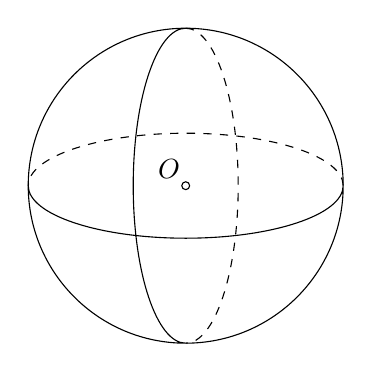
\begin{tikzpicture}
		\def\r{2}
		\path (0:0) coordinate (O);
		\draw[dashed] (0:\r) arc (0:180:{\r} and {\r/3}) (90:\r) arc (90:-90:{\r/3} and {\r});
		\draw (O) circle (\r) (180:\r) arc (180:360:{\r} and {\r/3}) (90:\r) arc (90:270:{\r/3} and {\r});
		\foreach \x/\g in {O/135} \draw[fill=white] (\x) circle (.05) + (\g:.3) node{$\x$};
	\end{tikzpicture}
\end{center}
\fbox{1} Quay nửa hình tròn tâm $O$ 1 vòng quanh đường kính $AB$ cố định ta được 1 hình cầu. \fbox{2} {\sf Thiết diện}: Cắt hình cầu (mặt cầu) bán kính $R$ bởi 1 mặt phẳng ta được 1 hình tròn (đường tròn) bán kính $r$: Bán kính đường tròn lớn $r = R$ nếu mặt phẳng cắt đi qua tâm. Bán kính đường tròn $r < R$ nếu mặt phẳng cắt không đi qua tâm. \fbox{3} Hình cầu có diện tích \fbox{$S = 4\pi R^2 = \pi d^2$}, thể tích \fbox{$V = \frac{4}{3}\pi R^3$}. \fbox{4} Hình cầu nội tiếp hình trụ thì bán kính hình cầu bằng bán kính đáy hình trụ, chiều cao hình trụ bằng đường kính hình cầu, $V_{\rm c} = \frac{2}{3}V_{\rm tr}$. \fbox{5} {\sf Công thức tính thể tích các vật thể có 2 đáy song song}: \fbox{$V = \dfrac{h}{6}(B_1 + 4B_2 + B_3)$} với $h$: chiều cao của vật thể, $B_1$: diện tích đáy dưới, $B_2$: diện tích thiết diện trung bình (thiết diện qua trung điểm của chiều cao), $B_3$: diện tích đáy trên.\\
\\
\cite[Chap. X, \S3, pp. 104--108]{SGK_Toan_9_Canh_Dieu_tap_1}: HD1. HD2. LT1. HD3. HD4. LT2. HD5. 1. 2. 3. 4.

\begin{baitoan}[{\sf Program}: Sphere]
	Cho 1 trong 4 yếu tố: $R,d,S,V$, tìm 3 yếu tố còn lại của hình cầu theo yếu tố cho trước. Viết chương trình {\sf Pascal, Python, C{\tt/}C++} để minh họa.
\end{baitoan}

\begin{baitoan}[\cite{Binh_boi_duong_Toan_9_tap_2}, H1, p. 125]
	Khi bán kính 1 mặt cầu tăng gấp $3,a$ lần thì diện tích mặt cầu \& thể tích hình cầu tăng lên mấy lần?
\end{baitoan}

\begin{baitoan}[\cite{Binh_boi_duong_Toan_9_tap_2}, H2, p. 125]
	1 hình cầu có thể tích $V = 36\pi\ {\rm cm}^3$. Tính độ dài đường tròn lớn.
\end{baitoan}

\begin{baitoan}[\cite{Binh_boi_duong_Toan_9_tap_2}, H3, p. 125]
	1 hình cầu có diện tích hình tròn lớn là $S = 144\pi\ {\rm cm}^2$. Tính thể tích hình cầu.
\end{baitoan}

\begin{baitoan}[\cite{Binh_boi_duong_Toan_9_tap_2}, H4, p. 125]
	1 hình cầu có thể tích $V = 40\ {\rm cm}^3$ nội tiếp 1 hình trụ. Tính thể tích hình trụ.
\end{baitoan}

\begin{baitoan}[\cite{Binh_boi_duong_Toan_9_tap_2}, VD1, p. 125]
	1 hình cầu nội tiếp 1 hình trụ. Chứng minh: (a) Diện tích mặt cầu bằng $\frac{2}{3}$ diện tích toàn phần của hình trụ. (b) Thể tích hình cầu bằng $\frac{2}{3}$ thể tích hình trụ.
\end{baitoan}

\begin{baitoan}[\cite{Binh_boi_duong_Toan_9_tap_2}, VD2, p. 126]
	1 hình nón có đường sinh bằng $l = 6$ \& có bán kính đáy bằng bán kính 1 hình cầu. Biết diện tích toàn phần của hình nón bằng diện tích mặt cầu. Tính: (a) Bán kính hình cầu. (b) Diện tích mặt cầu \& thể tích hình cầu.
\end{baitoan}

\begin{baitoan}[\cite{Binh_boi_duong_Toan_9_tap_2}, VD3, p. 126]
	1 trái bưởi hình cầu có lớp vỏ dày $a = 1$ {\rm cm}. Biết thể tích của lớp vỏ là $V = 909\ {\rm cm}^3$. Tính thể tích của các múi bưởi.
\end{baitoan}

\begin{baitoan}[\cite{Binh_boi_duong_Toan_9_tap_2}, VD4, p. 127]
	1 bình thủy tinh hình trụ đang chứa nước, có đường kính bên trong của đáy là $r = 6$ {\rm cm} \& ngập hoàn toàn trong nước làm mực nước trong bình dâng lên (nhưng chưa tràn ra ngoài). Mực nước trong bình dâng cao thêm nhiêu?
\end{baitoan}

\begin{baitoan}[\cite{Binh_boi_duong_Toan_9_tap_2}, VD5, p. 127]
	1 hình nón có bán kính đáy $R = 6$, chiều cao $h = 8$. 1 hình cầu nội tiếp hình nón đó. Chứng minh hình cầu này có số đo diện tích mặt cầu $\rm m^2$ bằng số đo thể tích của nó $\rm m^3$.
\end{baitoan}

\begin{baitoan}[\cite{Binh_boi_duong_Toan_9_tap_2}, 10.1., p. 128]
	1 hình cầu có số đo thể tích $\rm cm^3$ bằng k lần số đo diện tích $\rm cm^2$. Chứng minh bán kính hình cầu là $3k$ {\rm cm}.
\end{baitoan}

\begin{baitoan}[\cite{Binh_boi_duong_Toan_9_tap_2}, 10.2., p. 128]
	Vĩ độ của thủ đô Hà Nội là $21^\circ$ Bắc. Tính độ dài của vĩ tuyến qua Hà Nội, biết bán kính Trái Đất là $R_{\rm earth} = 6370$ {\rm km}. Mở rộng cho vĩ độ $a^\circ$.
\end{baitoan}

\begin{baitoan}[\cite{Binh_boi_duong_Toan_9_tap_2}, 10.3., p. 128]
	1 hình nón có nửa góc phẳng ở đỉnh bằng $30^\circ$. Chứng minh diện tích toàn phần của nó bằng diện tích mặt cầu có đường kính bằng chiều cao hình nón.
\end{baitoan}

\begin{baitoan}[\cite{Binh_boi_duong_Toan_9_tap_2}, 10.4., p. 128]
	1 hình cầu nội tiếp 1 hình lập phương. Chứng minh tỷ số giữa thể tích hình cầu \& thể tích hình lập phương đúng bằng tỷ số giữa diện tích mặt cầu \& diện tích toàn phần của hình lập phương.
\end{baitoan}

\begin{baitoan}[\cite{Binh_boi_duong_Toan_9_tap_2}, 10.5., p. 128]
	Cho hình cầu tâm O, bán kính $R = 20$. Cắt hình cầu bởi 1 mặt phẳng ta được 1 hình tròn tâm K, với AB là 1 đường kính. (a) Biết $OK = a = 12$, tính bán kính của hình tròn tâm K. (b) Tính tỷ số $\%$ giữa diện tích của hình tròn tâm K \& diện tích mặt cầu.
\end{baitoan}

\begin{baitoan}[\cite{Binh_boi_duong_Toan_9_tap_2}, 10.6., p. 128]
	Cho hình cầu tâm O, bán kính OA. Cắt hình cầu bởi 1 mặt phẳng vuông góc với OA ta được 1 hình tròn tâm M, có diện tích $s = 81\pi\ {\rm cm}^2$. Nếu cắt hình cầu này bởi 1 mặt phẳng đi qua tâm O ta được 1 hình tròn có diện tích là $S = 225\pi\ {\rm cm}^2$. (a) Tính thể tích hình cầu. (b) Tính thể tích hình nón đỉnh O, đáy là hình tròn tâm M.
\end{baitoan}

\begin{baitoan}[\cite{Binh_boi_duong_Toan_9_tap_2}, 10.7., p. 128]
	Cho tam giác đều cạnh a, đường cao AH. Quay đường tròn nội tiếp \& đường tròn ngoại tiếp tam giác đều này 1 vòng quanh AH cố định. Tính: (a) Tỷ số diện tích 2 mặt cầu nội tiếp \& ngoại tiếp hình nón. (b) Tỷ số thể tích 2 hình cầu.
\end{baitoan}

\begin{baitoan}[\cite{Binh_boi_duong_Toan_9_tap_2}, 10.8., p. 128]
	Cho nửa đường tròn $(O)$ đường kính $AB = d = 12$. Trên đường kính AB lấy điểm M. Vẽ vào trong nửa đường tròn đã cho các nửa đường tròn đường kính AM,BM. Quay toàn bộ hình vẽ 1 vòng quanh đường kính AB cố định ta được 3 hình cầu. Tìm thể tích lớn nhất của phần không gian được giới hạn bởi 3 hình cầu.
\end{baitoan}

\begin{baitoan}[\cite{Tuyen_Toan_9_old}, VD31, p. 163]
	1 vật nặng hình cầu rơi xuống 1 nền cát phẳng để lại 1 vết lõm hình chảo có đường kính {\rm72 cm} \& nơi sâu nhất là {\rm24 cm}. Tính thể tích của vật hình cầu đó.
\end{baitoan}

\begin{baitoan}[\cite{Tuyen_Toan_9_old}, 166., p. 164]
	Chứng minh diện tích mặt cầu bằng $\frac{2}{3}$ diện tích toàn phần hình trụ ngoại tiếp nó.
\end{baitoan}

\begin{baitoan}[\cite{Tuyen_Toan_9_old}, 167., p. 164]
	1 mặt phẳng cắt 1 hình cầu bán kính R theo 1 hình tròn có diện tích bằng $\frac{3}{16}$ diện tích mặt cầu. Tính khoảng cách từ tâm mặt cầu đến mặt phẳng cắt.
\end{baitoan}

\begin{baitoan}[\cite{Tuyen_Toan_9_old}, 168., p. 165]
	1 vật hình cầu nằm trên mặt sân bằng phẳng. Tại 1 thời điểm có ánh nắng mặt trời, bóng của quả cầu cách tiếp điểm của quả cầu trên mặt sân là {\rm6 m}, trong khi đó 1 chiếc cọc đóng vuông góc với mặt sân, cao {\rm1 m} có bóng dài {\rm0.75 m}. Tính thể tích khối cầu.
\end{baitoan}

\begin{baitoan}[\cite{Tuyen_Toan_9_old}, 169., p. 165]
	1 hình nón có đỉnh là tâm 1 hình cầu, có đáy là hình tròn tạo bởi 1 mặt phẳng cắt hình cầu. Biết diện tích đáy hình nón là $441\pi\ {\rm cm}^2$, thể tích của nó là $2940\pi\ {\rm cm}^3$. Tính diện tích mặt cầu.
\end{baitoan}

\begin{baitoan}[\cite{Tuyen_Toan_9_old}, 170., p. 165]
	Cho $\Delta ABC$ vuông tại A có $BC = 2a,\widehat{B} = 30^\circ$. Quay tam giác vuông này 1 vòng quanh AB được 1 hình nón đỉnh B. Chứng minh: (a) Diện tích toàn phần của hình nón bằng diện tích mặt cầu có đường kính AB. (b) Thể tích hình nón bằng $\frac{2}{3}$ thể tích hình cầu đường kính AB.
\end{baitoan}

\begin{baitoan}[\cite{Binh_Toan_9_tap_2}, VD48, p. 117]
	Có $15$ quả bi-a hình cầu đặt nằm trên mặt bàn, sao cho chúng được dồn khít trong 1 khung hình tam giác đều có chu vi bằng {\rm858 mm}. Tính bán kính của mỗi quả bi-a.
\end{baitoan}

\begin{baitoan}[\cite{Binh_Toan_9_tap_2}, 352., p. 117]
	1 quả bóng hình cầu bán kính {\rm13 cm} nổi trên mặt hồ, đỉnh của quả bóng cao hơn mặt hồ {\rm18 cm}. Tính độ dài của đường tròn được tạo thành bởi quả bóng \& mặt hồ.
\end{baitoan}

\begin{baitoan}[\cite{Binh_Toan_9_tap_2}, 353., p. 117]
	1 quả bóng hình cầu đặt trên mặt đất có bóng là 1 hình elip với độ dài lớn nhất của bóng là {\rm1 m}. Biết 1 cột cao {\rm1 m} lúc đó có bóng dài {\rm2 m}, tính bán kính quả bóng.
\end{baitoan}

\begin{baitoan}[\cite{Binh_Toan_9_tap_2}, 354., pp. 117--118]
	1 hình cầu nội tiếp 1 hình trụ, i.e., hình cầu được đặt khít vào trong hình trụ. Tính: (a) Tỷ số giữa diện tích mặt cầu \& diện tích toàn phần hình trụ. (b) Tỷ số giữa thể tích hình cầu \& thể tích hình trụ.
\end{baitoan}

\begin{baitoan}[\cite{Binh_Toan_9_tap_2}, 354., p. 117]
	Cho hình hộp chữ nhật $ABCD.A'B'C'D'$. (a) Chứng minh tồn tại 1 hình cầu đi qua tất cả các đỉnh của hình hộp chữ nhật. (b) Tính thể tích của hình cầu đó biết 3 kích thước của hình hộp chữ nhật là: (i) $6,8,26$. (ii) $a,b,c > 0$.
\end{baitoan}

%------------------------------------------------------------------------------%

\section{Miscellaneous}
\cite[BTCCX, pp. 109--110]{SGK_Toan_9_Canh_Dieu_tap_1}: 1. 2. 3. 4. 5. 6. 7.

\begin{baitoan}[\cite{Tuyen_Toan_9_old}, VD32, p. 165]
	Cho nửa đường tròn $(O;R)$ đường kính AB. Vẽ 2 tia tiếp tuyến $Ax,By$ cùng phía với nửa đường tròn đã cho. Trên tia Ax lấy điểm C sao cho $AC = x\le R$. Từ C vẽ 1 tiếp tuyến thứ 2 với nửa đường tròn, tiếp xúc với nửa đường tròn tại M, cắt By tại D. (a) Tính BD theo $R,x$. (b) Tính diện tích nhỏ nhất của tứ giác ABDC. (c) Quy hình vẽ 1 vòng quanh trục AB. Tính x để tổng thể tích 2 hình nón đỉnh O có đáy lần lượt là 2 hình tròn có bán kính $AC,BD$ đúng bằng thể tích của hình cầu đường kính AB.
\end{baitoan}

\begin{baitoan}[\cite{Tuyen_Toan_9_old}, 171., p. 167]
	1 bồn chứa xăng dầu có phần dưới là 1 hình trụ mà chiều cao bằng đường kính đáy \& phần trên là 1 bán cầu có đường kính bằng đường kính hình trụ. Biết diện tích toàn phần của bồn chứa là $445\ {\rm cm}^2$, tính thể tích của nó.
\end{baitoan}

\begin{baitoan}[\cite{Tuyen_Toan_9_old}, 172., p. 167]
	Cho hình cầu $(O;R)$ đường kính AB. M là trung điểm OB. Mặt phẳng qua M \& vuông góc với AB cắt hình cầu theo 1 hình tròn $(M)$. (a) Tính thể tích hình nón đỉnh A đáy là thiết diện hình tròn $(M)$. (b) 1 hình cầu nội tiếp hình nón này. Tính tỷ số diện tích mặt cầu này với diện tích hình tròn lớn của hình cầu $(O;R)$.
\end{baitoan}

%------------------------------------------------------------------------------%

\printbibliography[heading=bibintoc]
	
\end{document}